\section{Jet}
\label{sec:jet} 
\subsection{Reconstruction}
\large
A jet can be defined as a collimated spray 
of stable particles arising from the fragmentation
and hadronisation of a parton (quark or gluon) after a collision.
Jets provide a link between the observed colourless 
stable particles and the underlying physics at the partonic
level. A basic illustration of a collision of two protons,
the subsequent particle shower and a reconstructed jet is 
shown in Figure~\ref{fig:jets}.

\begin{figure}[bht]
    \begin{centering}	
    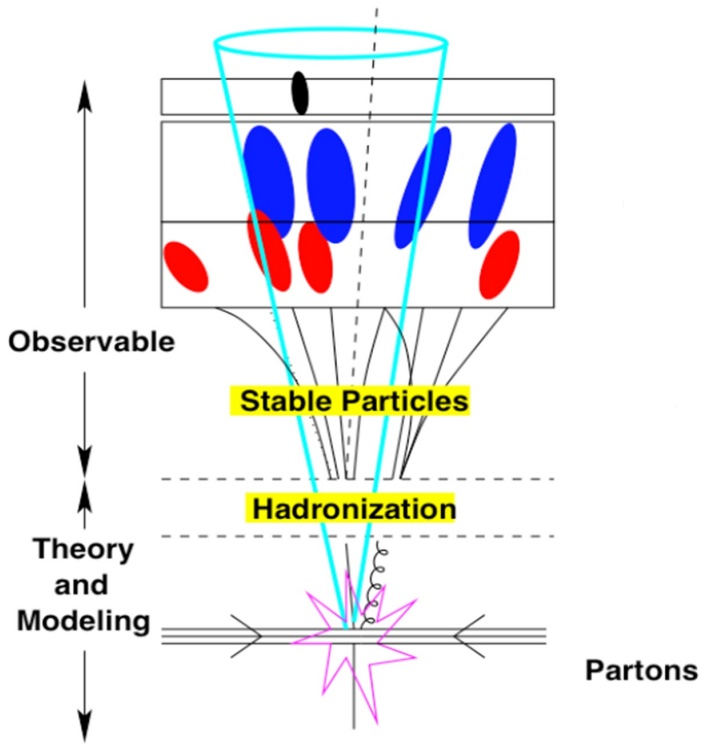
\includegraphics[width=.6\textwidth]{Reconstruction_plots/Jets.jpg}
    \caption{A simple example of an event showing the point of collision, 
    the fragmentation and hadronization of the quarks and gluons and the 
    resulting jet found through the detection of the stable particles. 
    Image reproduced from~\cite{atkin2015review}.
        }
    \label{fig:jets}
    \end{centering}
\end{figure}

The jet reconstruction starts by forming clusters of energy deposit
in the calorimeters performing a three-dimensional topological clustering 
of individual calorimeter cell signals~\cite{Aad_2017}.
The algorithm clusters the energy deposits into so called ``topo-clusters'' 
and combines their four-momenta. 
In Run 1 of the LHC, the ATLAS experiment used either
solely the calorimeter or solely the tracker to reconstruct
hadronic jets and soft particle activity, 
and the vast majority of analysis utilised jets that were built 
from topo-clusters, referred to \textit{EMTopo jets}.
% These jets were then calibrated to the particle level using a jet energy scale
% (JES) correction factor [4–7]. For the final Run 1 jet calibration, this correction factor also took into account the tracks
% associated with the jet, as this was found to greatly improve
% the jet resolution [4]. 
An alternative approach called ``\textit{Particle flow}'' (PFlow) was done
in ATLAS, as described in details in reference~\cite{PERF-2015-09}. 
It is the default approach for the thesis.
Measurements from both the tracker and the calorimeter 
are combined to form the signals. 
More specifically, the algorithm matches the reconstructed tracks
to the candidate leptons and hadrons, in oder to produce a new
set of clusters called \textit{PFlow clusters} from topo-clusters.
% The energy deposited in the calorimeter by all the charged particles is removed.
% Jet reconstruction is then performed on topo-clusters
% consisting of the remaining calorimeter energy and 
% tracks which are matched to the hard interaction.
% The main advantages of integrating tracking and calorimetric information 
% into one hadronic reconstruction step is that for 
% low-energy charged particles, the momentum resolution of the tracker is significantly
% better than the energy resolution of the calorimeter (see Table \ref{tab:ATLAS_performance}).
% Above $p_T^{track}$ = 100 GeV no track information is used as the PFlow algorithm 
% becomes equivalent to EMTopo benefitting from excellent
% calorimeter performance at high energies.
% In addition, with track reconstructed, one can ascertain whether it is 
% associated with a vertex. This information can be used to mitigate 
% in-time pileup signals. 
Using the PFlow clusters as inputs, PFlow jets are then reconstructed
using the anti-$k_t$ algorithm~\cite{Cacciari_2008}. 
% The inputs to jet reconstruction are 
% the tracks that are matched to the primary vertex,
% and positive energy topo-clusters which survives the energy subtraction step 
% and matches to the selected tracks. 
The anti-$k_t$ algorithm 
sequentially combines PFlow clusters into larger clusters based on the 
momentum-weighted distance between clusters. 
For two clusters $i$ and $j$ the algorithm defines:
\[  d_{i,j} = min(p_{T,i}^{2p},p_{T,j}^{2p}) \frac{\Delta R_{i,j}^2}{R^2} \]
and 
\[ d_{i,beam} = p_{T,i}^{2p} \]
where $p$ is a exponent parameter and the value of -1 is used
for the anti-$k_t$ algorithm (as the name `anti' suggests),
$\Delta R^2{i,j} = (\eta_i - \eta_j)^2 + (\phi_i - \phi_j)^2 $, 
and $p_{T,i}$, $\eta_i$ and $\phi_i$ are 
the transverse momentum, 
pseudorapidity and azimuthal coordinate
of cluster $i$, respectively. 
The parameter $R$ controls the size of the jet and for standard jets 
in ATLAS this is chosen to be $R$ = 0.4.
The algorithm combines objects $i$, $j$ with minimum value of $d_{i,j}$
into one object iterartively, until no more $d_{i,j}$ can be found greater
than $d_{i,beam}$, where the combined object is considered the final jet 
candidate.
% The algorithm calculates $d_{i,j}$ iterartively for all clusters: 
% when $d_{i,j} < d_{i,beam}$, the two clusters $i$, $j$ are combined
% into a single cluster, and the new cluster is added back to the list
% of consideration; when $d_{i,j} > d_{i,beam}$, the cluster $i$ is 
% considered final jet candidate and it is removed from the list of clusters.
% The anti-$k_t$ algorithm uses $p$ = -1 (as the name `anti' suggests), 
% which means that algorithm is more likely to combine two clusters with 
% very close to each other (as a result of the $\frac{\Delta R_{i,j}^2}{R^2}$ term)
% or cluster having large \pt\ with clusters having smaller \pt\ (as a result of
% the $min(p_{T,i}^{2p},p_{T,j}^{2p})$ term). 

A validation study is done by the author for comparison of the EMTopo jets 
to PFlow jets used in the analysis TODO: add reference after selection is defined.

\subsection{Calibration}
After the jets are reconstructed, the four-momenta of jets
are calibrated with the jet energy scale (JES) calibration
consists of several consecutive stages derived from a
combination of MC-based methods and in situ techniques \cite{PERF-2016-04}.
MC-based calibrations correct the reconstructed jet four momentum 
to that found from the simulated stable particles 
within the jet. 
The calibrations account for features of the
detector, the jet reconstruction algorithm, jet fragmentation,
and the busy data-taking environment resulting from multiple $pp$ 
interactions, and the difference in jet response between
data and MC simulation.
In order to calibrate jet energy resolution (JER),
jet momentum must be measured precisely. 
As described in details in reference \cite{JETM-2018-05},
a \textit{dijet balance} approach is used for this purpose with well-defined dijet system,
where the two jets are expected to have \pt\ that sum up to 0 precisely.
Furthermore, jets arised from pileup are suppressed by using the 
\textit{jet vertex tagger}, which is a multivariate 
combination of track-based variables developed to separate 
hard-scatter jets from pileup jets~\cite{ATLAS-CONF-2014-018}.
A jet cleaning selection is applied in order to veto any `fake' jets, 
which arise from non-collision background events, such as cosmic rays, 
or from detector effects. 
Finally, all jets in the analysis are required to have \pt\ < 20 GeV 
and $|\eta|$ < 2.5.


\subsection{Identification of heavy quark flavoured jets}
\label{sec:Flavour tagging}
As frequently being called \textit{flavour tagging}, 
the identification of jets containing $b$-hadrons (\bjets) 
against the large background of jets containing $c$-hadrons 
(\cjets) or jets coming from the hadronization of light ($u$,$d$,$s$) 
quarks or gluons (light jets) is of major importance in many areas of the 
physics programme of the ATLAS experiment at the LHC. 
It is crucial in a large number of SM
precision measurements, studies of the Higgs boson properties, 
searches for new phenomena~\cite{SUSY-2014-08, ATLAS-CONF-2018-043,Interpreting_Higgs_result},
and it also plays an important role in 
the $HH \to bb\tau\tau$ searches presenting in Chapter \ref{sec:search for dihiggs}. 

% as well as the recent 
% observation of the Higgs boson decay into bottom quarks~\cite{HIGG-2018-04} 
% and of its production in association with a top-quark pair~\cite{HIGG-2018-13}. 


The ATLAS Collaboration uses various algorithms to identify 
\bjets~\cite{PERF-2012-04}, referred to as \btagging\ algorithms, 
when analysing data recorded during Run 2 of the LHC. These 
algorithms exploit the long lifetime, high mass and high decay 
multiplicity of $b$-hadrons, as well as the properties of the \bquark\  
fragmentation. Given a lifetime of the order of 1.5 ps, $b$-hadrons have a 
significant mean flight length ($\langle c\tau \rangle$ $\approx$ 450 $\mu m$), 
in the detector before decaying, generally leading to at least one vertex 
displaced from the hard-scatter collision point, as illustrated in Figure~\ref{fig:b-jet-decay}.

\begin{figure}[bth]
	\begin{centering}	
	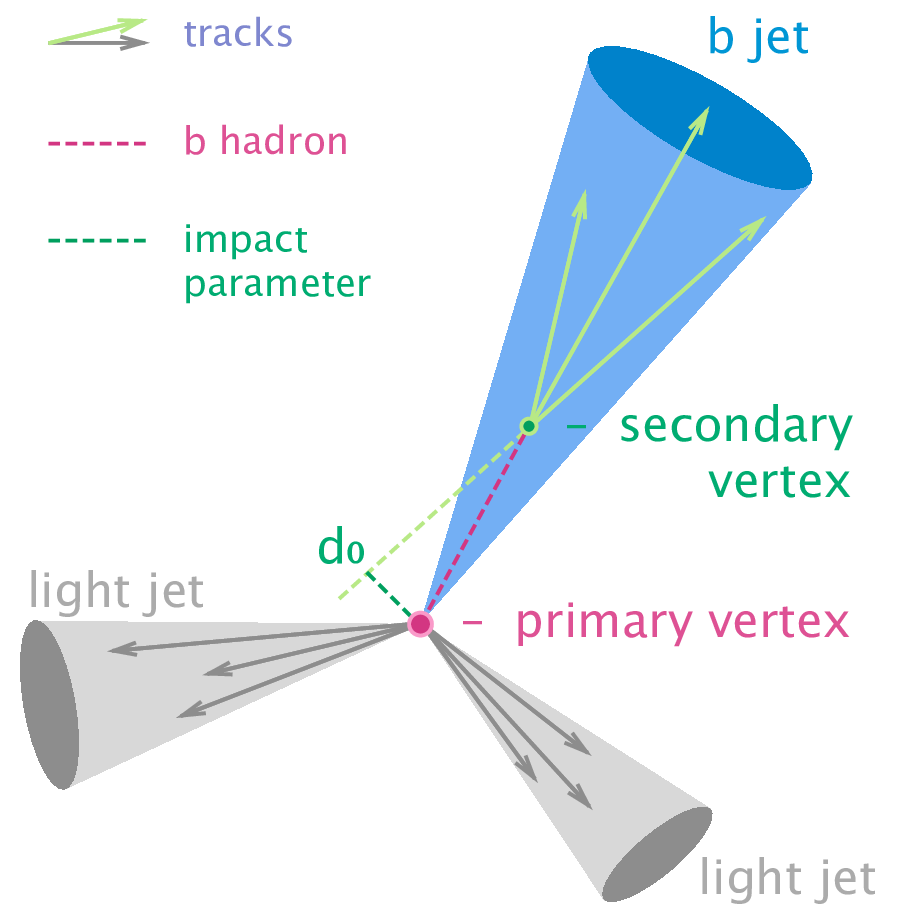
\includegraphics[width=.6\textwidth]{FTAG_plots/B-tagging_diagram.png}
	\caption{A diagram showning the b hadron decay initiated jets. }
	\label{fig:b-jet-decay}
	\end{centering}
\end{figure}


The strategy developed by the ATLAS Collaboration is based on a two-stage approach. 
Firstly, low-level algorithms reconstruct the characteristic features of 
the \bjets\ via two complementary approaches, a) that uses the 
individual properties of charged-particle tracks
associated with a hadronic jet, and b) that 
combines the tracks to explicitly reconstruct displaced vertices. 
These algorithms, first introduced during Run 1~\cite{PERF-2012-04}, 
have been improved and retuned for Run 2~\cite{FTAG-2018-01}. 
Secondly, in order to 
maximise the \btagging\ performance, the results of the low-level 
\btagging\ algorithms are combined into high-level algorithms 
via multivariate classifiers. 


The most performant algorithms presently in use in physics 
analyses at ATLAS are based on multivariate combinations 
of the available information (MV2) or additionally using a
deep feed-forward neural network (DL1)~\cite{tagging,ATL-PHYS-PUB-2017-013}, 
as shown in Figure~\ref{fig:b-tagging-performance}, where the performance
is characterised by the probability of 
tagging a \bjet\ (\bjet\ tagging efficiency, 
$\epsilon_b$) and the probability of mistakenly identifying 
a \cjet or a light-flavour jet as a \bjet\, 
labelled $\epsilon_c$($\epsilon_l$). 
In addition, the distribution of the output discriminant
of the MV2 and DL1 tagger for \bjet, \cjet, and light-flavour jets
in the \ttbar\ simulated events are shown in Figure~\ref{fig:b-tagging-score}.
Depending on the low-level algorithm, 
the DL1 tagger can be further separated into two taggers: DL1 and DL1r,
where the DL1 tagger uses traditional track-based impact parameter 
taggers IP2D and IP3D~\cite{ATL-PHYS-PUB-2016-012} 
and the DL1r tagger uses a Recurrent Neural Network Impact Parameter tagger 
(RNNIP)~\cite{ATL-PHYS-PUB-2017-013}. 
The calibration of DL1 and DL1r algorithms has been an original contribution 
of the author of this thesis and it is described in more detail in Chapter~\ref{sec:FTAG}.
The DL1r tagger is now the 
default \btagging\ algorithm used for flavour tagging in ATLAS.
% where performance of the algorithms is quantified 
% in terms of \bjet\ efficiency versus \cjet\ (light jet) rejections, defined as 
% 1/$\epsilon_c$ and 1/$\epsilon_l$. 


%Their high mass also leads to decay products with a larger transverse momentum relative to the jet axis with respect to the ones typically found in jets from light partons. Finally, heavy hadrons have a sizable branching ratio for semileptonic decays, hence the presence of soft leptons in the produced jets provides another tool for heavy jet identification. %The general strategy is to start with simple algorithms that exploits a particular property of b jets and progressively add more information to build moresophisticated algorithms. %The output of these algorithms consists in a discriminant value for each jet. Operating points are then defined as thresholds on the discriminant, designed to provide a determined efficiency for identifying b jets.
% Low-level $b$-taggingalgorithms fall into two broad categories. A first approach, implemented in the IP2D and IP3D algorithms~\cite{ATL-PHYS-PUB-2017-013}, or RNNIP~\cite{ATL-PHYS-PUB-2017-003} is inclusive and based on exploiting the large impact parameters of the tracks originating from the $b$-hadron decay. The second approach explicitly reconstructs displaced vertices. To maximise the $b$-tagging performance, low-level algorithm results are combined using multivariate classifiers. To this end, two high-level tagging algorithms have been developed. The first one,MV2\cite{ATL-PHYS-PUB-2017-013}, is based on a boosted decisiontree (BDT) discriminant, while the second one,DL1, is based on a deep feed-forward neural network(NN). These two algorithms are presented in fig .
\begin{figure}[bth]
	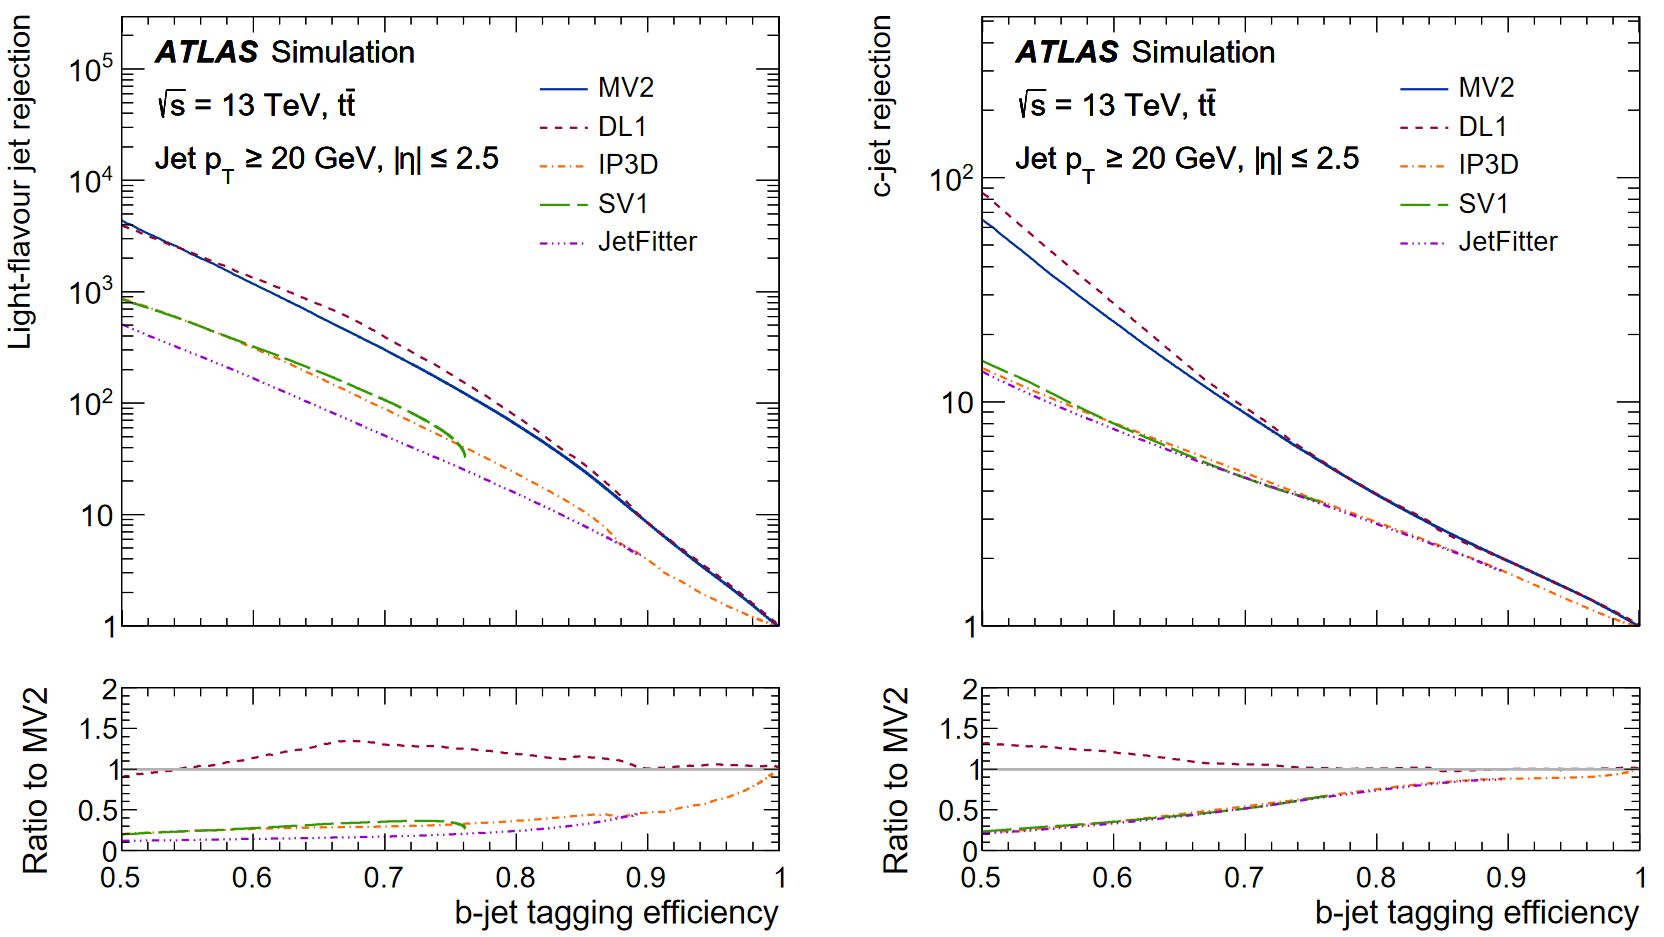
\includegraphics[width=.9\textwidth]{FTAG_plots/b-tagging-perfermance.png}
	\caption{The light-flavour jet (left) and \cjet\ (right) rejections versus 
	the \bjet\ tagging efficiency for the IP3D, SV1, JetFitter, MV2 and
	DL1 b-tagging algorithms evaluated on the \ttbar\ events
	~\cite{FTAG-2018-01}.}\label{fig:b-tagging-performance}
\end{figure}


\begin{figure}[bth]
	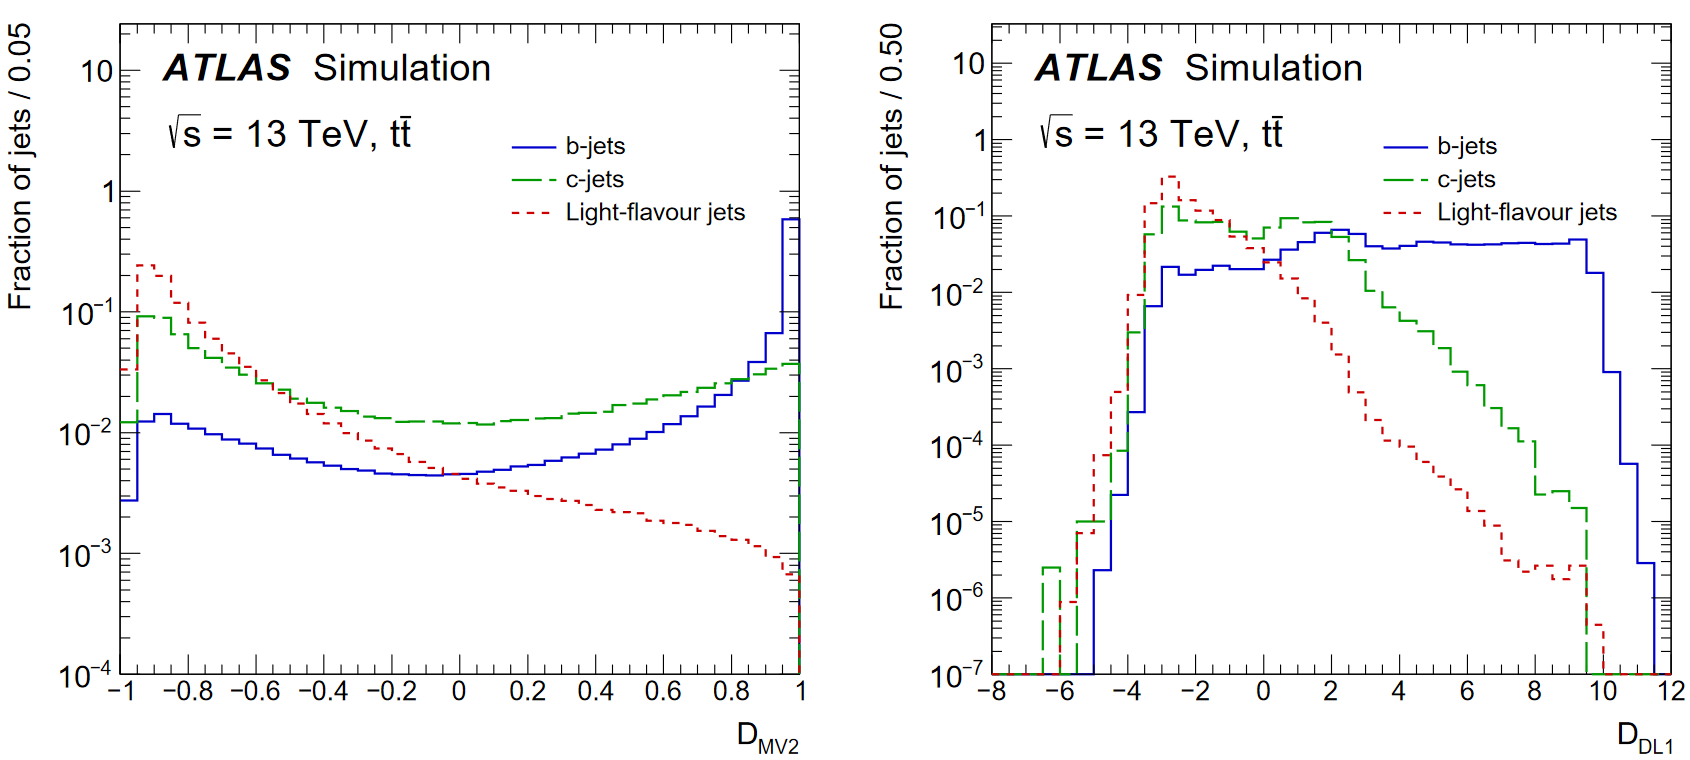
\includegraphics[width=.9\textwidth]{FTAG_plots/b-tagging-score.png}
	\caption{The fraction of light-flavour jets and \cjets\ versus 
	the \bjets\ in the MV2 (left) and
	DL1 (right) b-tagging algorithms output distribution 
	evaluated on the \ttbar\ events
	~\cite{FTAG-2018-01}.}\label{fig:b-tagging-score}
\end{figure}
